\documentclass[conference,10pt]{IEEEtran}
\usepackage[T1]{fontenc}
\usepackage{graphicx,booktabs,amsmath,amssymb,xcolor,url,xspace}
\usepackage[hidelinks]{hyperref}
\hypersetup{pdftitle={Replaying Hand-Worn-Gripper Demonstrations on a Bimanual Robot}, pdfauthor={Jeong Hwan Lee}}
\newcommand{\mm}{\,mm\xspace}
\DeclareMathOperator{\clip}{clip}
\begin{document}
\title{Replaying Hand-Worn-Gripper Demonstrations\\on a Bimanual Robot: A Technical Note}
\author{\IEEEauthorblockN{Jeong Hwan Lee}
\IEEEauthorblockA{Research overview, October 2026 (sanitized public version)}}
\maketitle

\begin{abstract}
We want a two-arm robot to manipulate garments from human demonstrations recorded with hand-worn grippers, and first ask
a narrower question: if the robot simply replays the converted human motion, open loop, does it do what the human did?
Replay serves as an end-to-end test of calibration, pose recovery, jaw labelling and conversion before any policy is
trained. The demonstrator wears two HandUMI grippers (an open-source design by BrikHMP18, not ours) with AprilTags, wrist
fisheye cameras and IMUs; a fixed RGB-D camera observes the tags. With one world frame (the robot base) and one host
clock, single-arm replays reach 5.5--11.6\mm median per-axis RMSE, one arm grasped and lifted a T-shirt from human data,
and full two-arm replays of a 33\,s demonstration repeat within about 1\mm, close the jaws 5--19\mm above the table
(human $\approx$10\mm), and deviate by 17\mm (right) and 30\mm (left) RMSE from the robotized path that was replayed (22 and 32--34\mm from the raw human path). The robot does not yet fold
like the human, and we report no success rate. Wrist-camera SLAM was rejected as the pose source because it loses
tracking exactly at grasps.
\end{abstract}

\section{Introduction}
Hand-held and hand-worn grippers in the style of UMI~\cite{chi2024umi} let a person demonstrate with an end-effector that
resembles the robot's, without a robot in the loop. The cost moves into the conversion: every calibration, pose,
labelling, timing and feasibility error ends up in the training labels. We therefore test the data by replay first.
Replay exercises every stage at once, lets errors be attributed to a stage when human, command and robot share one
frame and one clock, and fails visibly. Contributions: (i) a shared robot-base world frame for human and robot set once
by calibration, without per-take alignment; (ii) a conversion from recording to robot-feasible jaw-tip trajectories with
jaw labels and per-frame quality; (iii) measured replay results, including negative ones.

\section{Related Work}
UMI~\cite{chi2024umi} obtains gripper pose from ORB-SLAM3-based~\cite{campos2021orbslam3} monocular-inertial SLAM and
filters trajectories by robot kinematics. HandUMI~\cite{handumi,meza2026handumi} is an open-source hand-worn variant for
robot-free bimanual capture; we use a build of it. DexUMI~\cite{xu2025dexumi} and EgoMimic~\cite{kareer2025egomimic} use
human hands and egocentric video as data sources. ALOHA~\cite{zhao2023aloha} demonstrated low-cost bimanual manipulation
from teleoperation; SpeedFolding~\cite{avigal2022speedfolding} and FlingBot~\cite{ha2021flingbot} learn cloth
primitives. We keep the UMI-style gripper but take pose from fixed-camera fiducials~\cite{olson2011apriltag,wang2016apriltag2}
plus depth, warp rather than filter infeasible paths, and test the data by replay.

\section{System Overview}
\begin{figure*}[!t]
\centering
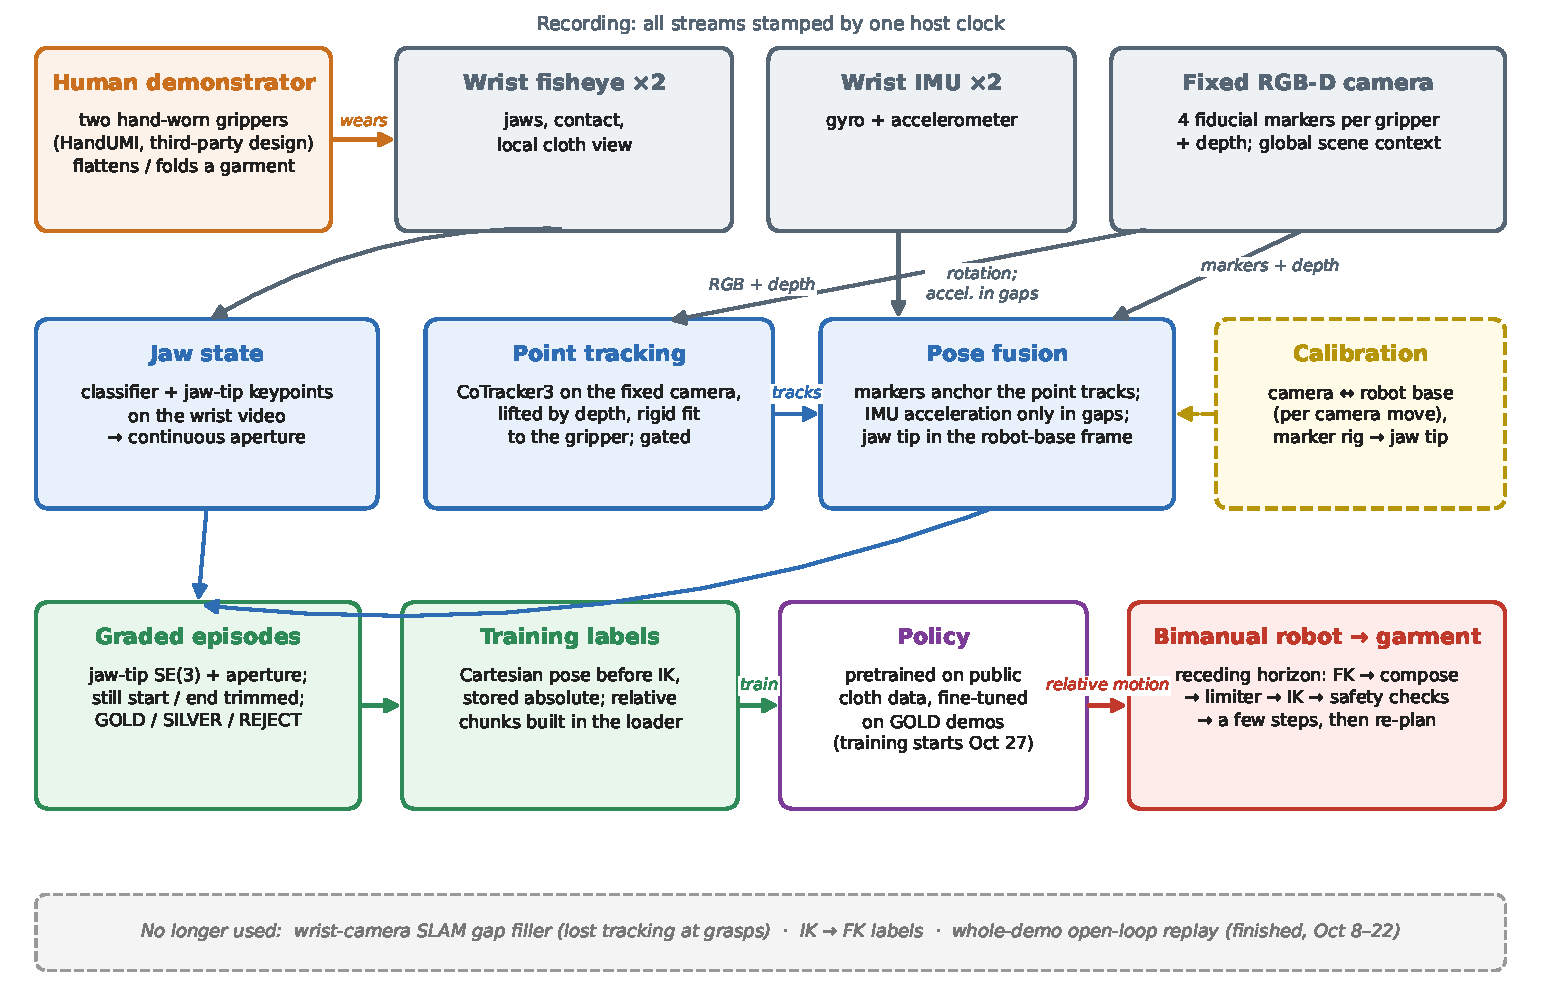
\includegraphics[width=0.86\textwidth]{../docs/architecture.pdf}
\caption{Data flow from the human demonstration to robot replay. Dashed: one-time calibration, the optional SLAM filler,
and future policy learning.}
\label{fig:pipe}
\end{figure*}
Figure~\ref{fig:pipe} shows the data flow. A fixed RGB-D camera, two wrist fisheye cameras and two wrist IMUs record the
demonstration; gripper poses are reconstructed in the robot base frame, completed by gap filling and paired with a jaw
state; the trajectory is robotized, planned and replayed, and human, command and robot are compared. Two principles run
through the system: \emph{one world frame} (Sec.~\ref{sec:world}) and \emph{one clock}: all streams, and later the
robot's commanded and measured joints, are stamped by one host clock, so no synchronisation hardware is needed.

\section{Hardware}
\begin{figure}[!t]
\centering
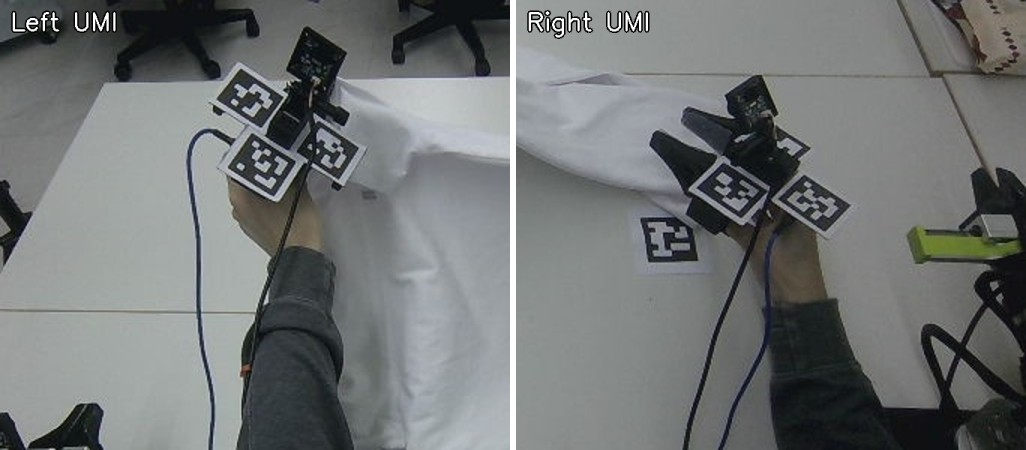
\includegraphics[width=\columnwidth]{figures/umi_hands.jpg}
\caption{The two hand-worn grippers (HandUMI, left and right) as used, each with three AprilTags.}
\label{fig:umi}
\end{figure}
The demonstrator wears two HandUMI grippers~\cite{handumi,meza2026handumi}, an open-source design by BrikHMP18 (not ours),
each with several AprilTags on different faces, a wrist fisheye camera and an IMU; the jaw servo was removed and the jaw
state is inferred from the wrist video (Fig.~\ref{fig:umi}). A fixed RGB-D camera about 1\,m above the table sees the
tags and the scene; two low-cost 6-DoF arms with parallel jaws replay.

\section{One World Frame for Human and Robot}\label{sec:world}
\begin{figure*}[!t]
\centering
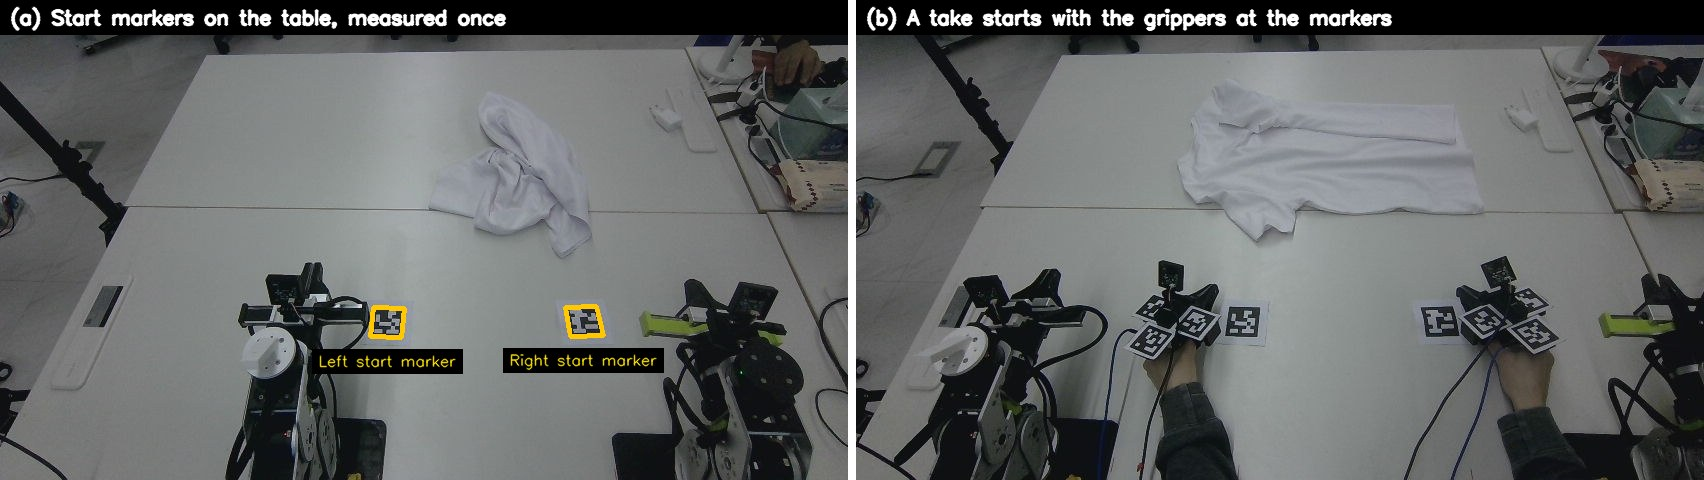
\includegraphics[width=0.8\textwidth]{figures/world_frame_start_markers.jpg}
\caption{(a) Start markers on the table, measured once in robot coordinates. (b) Every take starts with the grippers at
the markers.}
\label{fig:start}
\end{figure*}
All poses live in the robot base frame $B$. It is set up once per installation:
\begin{enumerate}
\item \emph{Camera to robot.} The robot moves a wrist-mounted tag through a set of poses in front of the camera, giving
  $T_{BC}$ (initialised with~\cite{shah2013robotworld}, refined on reprojection and depth residuals). From then on any
  camera measurement can be written in $B$.
\item \emph{Start markers.} Two tags on the table are measured in $B$ with the calibrated camera (Fig.~\ref{fig:start}a).
\item \emph{Gripper tags to jaw tip.} Each gripper's tags are calibrated to its jaw tip by touching known board corners
  (robust least squares), checked by an independent pivot test.
\item \emph{Start of every take.} Each take starts with the grippers at the start markers (Fig.~\ref{fig:start}b).
\end{enumerate}
No per-take alignment (SLAM map, point-cloud registration) is needed: a camera measurement of a gripper tag is already a
robot-frame pose.

\section{From Recording to Robot Motion}
\textbf{Pose.} Tags are solved with IPPE~\cite{collins2014ippe}; the tag range, the least accurate PnP coordinate, is
corrected along the ray by the median aligned depth. With several visible tags the gripper pose is solved jointly
(SQPnP~\cite{terzakis2020sqpnp} + Levenberg--Marquardt). Rotation may be stabilised by the gyroscope anchored to tag
frames. The jaw tip is $p_B=R_{BC}(R_{C,\mathrm{rig}}t_\mathrm{tcp}+p_{C,\mathrm{rig}})+t_{BC}$.

\textbf{Gaps and jaw state.} Tags vanish when the hand grasps palm-down. Short gaps get gyro rotation and interpolated
position and are flagged. MASt3R-SLAM~\cite{murai2025mast3rslam} on the wrist video is an optional filler, accepted per
segment only if a Sim(3) fit on alignment frames keeps it close to the tag path on held-out validation frames. An
ImageNet-pretrained~\cite{deng2009imagenet} ResNet-18~\cite{he2016resnet} per hand classifies the jaws in the wrist
fisheye.

\begin{figure*}[!t]
\centering
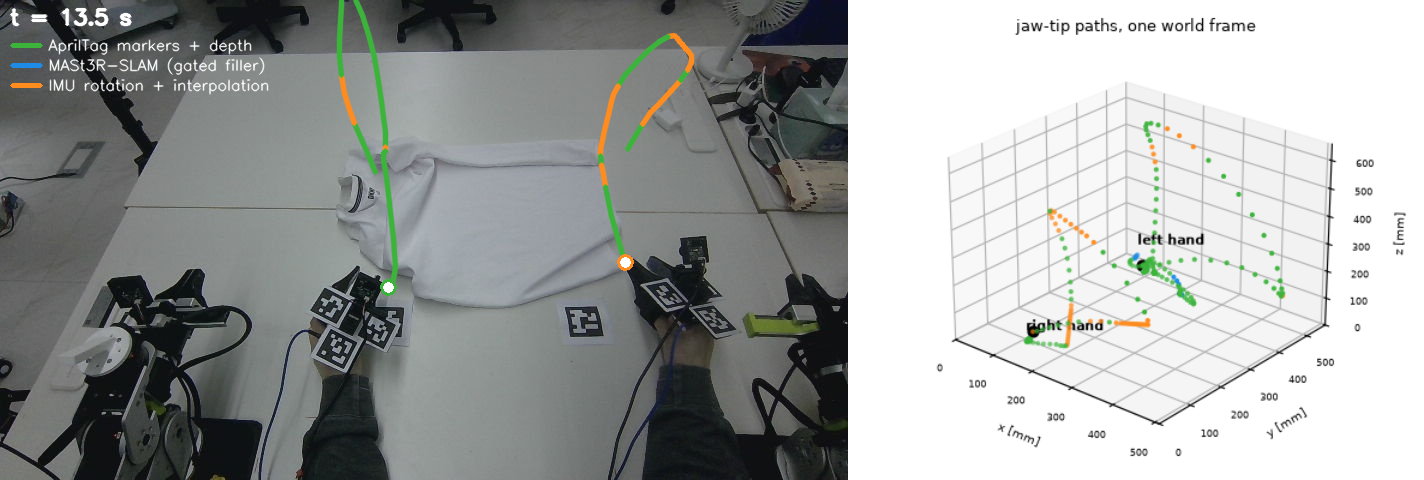
\includegraphics[width=0.86\textwidth]{figures/trajectory_sources.png}
\caption{Reconstructed jaw-tip trajectories of one demonstration (one frame of the animation in \texttt{media/}). Left: the
last 3\,s of both paths projected into the fixed camera, coloured by source: tags + depth (green), SLAM filler (blue), IMU
rotation + interpolation while tags are hidden (orange). Right: both paths in the robot base frame.}
\label{fig:traj}
\end{figure*}
Figure~\ref{fig:traj} shows which source supplies each frame: the orange (tag-hidden) parts occur exactly when a hand
grasps or lifts the cloth.

\textbf{Robotization.} The path is changed only by continuous warps. With $y_o,y_i$ the outer and inner lateral extent of
a hand and $d$ a minimum separation, the lateral coordinate is compressed toward the hand's own side and the height gets
a soft table floor:
\begin{align}
s&=\clip\big((-d/2-y_o)/(y_i-y_o),\,s_\mathrm{min},\,1\big),\\
y'&=\mathrm{softceil}\big(y_o+s(y-y_o),\,-d/2,\,w\big),\\
z'&=f+w\log\big(1+e^{(z-f)/w}\big).
\end{align}
Each frame stores its displacement and a quality class, intended as a label weight.

\textbf{Learning contract.} Absolute poses $T(t)$ are stored in $B$; learning targets will be relative,
$T_\mathrm{rel}(t)=T_0^{-1}T(t)$, identical for human and robot data.

\textbf{Planning and checks.} Differential IK with Pink~\cite{pink} on Pinocchio~\cite{carpentier2019pinocchio}:
position before orientation, joint limits, a bounded joint change per frame, wrist-roll relaxation about the tool axis,
use of the jaw's $180^\circ$ symmetry, and a finger-corner clearance model. Jaw commands lead the human events by the
measured actuation latency. Before execution the plan must pass IK error, joint limit and speed, TCP and link height,
and arm-to-arm distance checks.

\textbf{Evaluation.} A is the human (tags), B the command (FK of commanded joints), C the robot (FK of encoders). Each is
taken relative to the start of the window; C is shifted by the lag that best matches B. We report position RMSE/p95,
geodesic rotation error, amplitude ratio, C$-$B (tracking) and B$-$A (conversion and planning). Relative metrics hide
constant offsets, so absolute placement is checked separately by tape and by the same camera that films the human.

\section{Results}
\textbf{Calibration.} Camera-to-robot 0.98\,px held-out reprojection ($\approx$1.3\mm lateral); tag rig to jaw tip
1--4\mm static, 1.8--4.8\mm leave-one-out; corrected robot model within 6--9\mm of tape at the home pose. Two robot-model
errors of several centimetres (tool-centre point, one arm's mounting) were found only by measuring the real robot.

\textbf{Single-arm parity.} Translation strokes: 16/18 pass, median per-axis RMSE 5.5--11.6\mm. Rotation strokes:
geodesic median 0.3--1.6$^\circ$, amplitude ratio 0.98--1.04. Free motion: RMSE 13.7/14.6\mm. B$-$A $\le$3.4\mm, so the
residual was robot tracking. With an integral-only feed-forward and no gravity model, the moving error scales with the
rate of gravity-torque change over the integral gain, independent of the proportional gain; tuning the integral gain
reduced stroke RMSE from 25--37\mm to 12--14\mm.

\textbf{First cloth grasp.} One arm replayed a demonstration's grasp window and picked up and lifted the T-shirt.

\begin{table}[t]
\caption{Two-arm replay of one 33\,s demonstration vs.\ the replayed (robotized) path A (runs with one plan)}\label{tab:rep}
\centering\footnotesize\setlength{\tabcolsep}{4pt}
\begin{tabular}{@{}lccccc@{}}
\toprule
arm & RMSE & p95 & rot.\ med. & C$-$B & B$-$A \\
\midrule
right & 17.2--17.4\mm & 35--37\mm & 8.1$^\circ$ & 12\mm & 8.6\mm \\
left & 29.0--30.3\mm & 50--51\mm & 12.3--12.7$^\circ$ & 15\mm & 22.6\mm \\
\bottomrule
\end{tabular}
\end{table}

\begin{figure*}[!t]
\centering
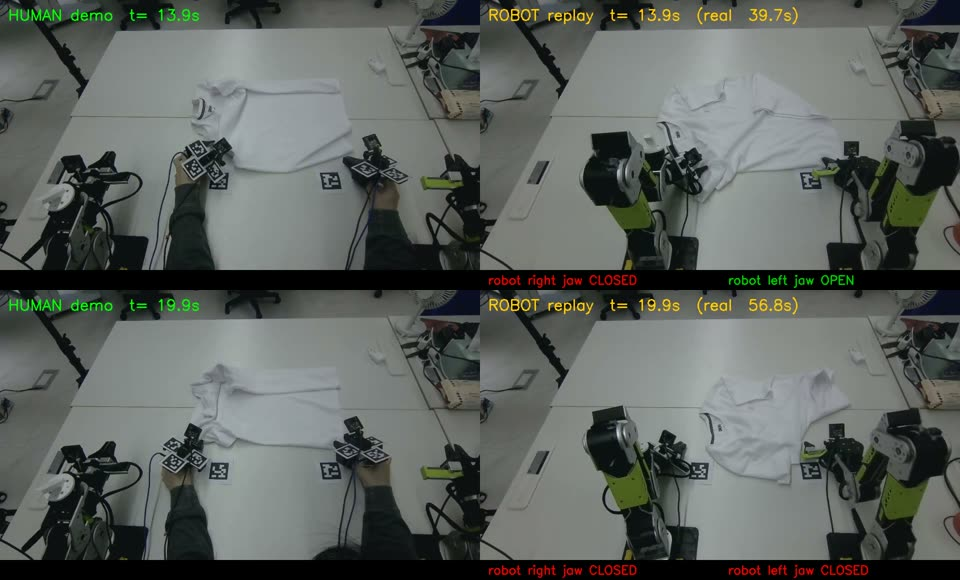
\includegraphics[width=0.66\textwidth]{figures/replay_frames.jpg}
\caption{Human demonstration (left) and robot replay of the converted trajectory (right), same fixed camera, aligned on one
clock; two moments of the 33\,s demonstration. The bar shows the robot jaw commands.}
\label{fig:replay}
\end{figure*}
\textbf{Two-arm replay.} In the demonstration, 79\,\% (right) and 95\,\% (left) of frames had a visible tag; robotization
moved frames by a median of 0.1/1.1\mm (p95 9.3/20.6\mm). Four runs of one plan agree within $\approx$1\mm
(Table~\ref{tab:rep}): the robot is deterministic and the error systematic. Against the raw human path the RMSE is
22\mm (right) and 32--34\mm (left), since the robotization displacement then counts as error; the left command also
deviates more from the replayed path (B$-$A). With a conservative finger-corner clearance the jaws closed 19--61\mm above the table and
missed the cloth; allowing the corner to touch the table plane, as human fingers do, gave 14--16\mm (right) and
5--19\mm (left), human $\approx$10\mm, within 2--8\mm of the command. Tilting the tool instead made the IK fail. In two
runs the shirt lay 15--20\,cm away and the jaws closed on the empty table; in one the jaws caught the shirt edge and
dragged it (Fig.~\ref{fig:replay}). The shirt was not folded.

\textbf{SLAM as the pose source (negative).} MASt3R-SLAM with restarts was accurate where it tracked (2--14\mm on held-out
tag frames) but kept only 19--48\,\% of frames and 0--38\,\% of tag-hidden frames near grasps. ORB-SLAM3 mono-inertial
diverged in scale (30--1000$\times$): hand accelerations (0.07--0.16\,m/s$^2$) were below the accelerometer bias. An earlier
SLAM-based label pipeline passed its own checks yet was 4--6\,cm off, which motivated the 1--4\mm tag rig.

\section{Lessons}
(1) Absolute tags plus depth beat wrist SLAM for contact-rich hand motion: SLAM's failure regime (close range,
textureless cloth, fast motion) is exactly the grasp. (2) Measure in the world, not in the model: model-vs-model parity
cannot see model errors. (3) Fix the conversion rather than adding heuristics. (4) One clock for everything removes the
need for synchronisation hardware. (5) Model the controller before tuning it. (6) Grade data with per-frame quality
instead of discarding it.

\section{Limitations and Next Steps}
No success rate: replays were judged by measurement and video. One demonstration was replayed in full; repeatability
shows determinism, not generality. Replay is open loop and needs the cloth where the human's was. Tag-hidden phases are
interpolated and their error at grasps is unmeasured. Jaw labels lack a held-out accuracy on demonstrations. Next: a
per-grasp error table (constant bias vs.\ varying error), a cloth-placement reference, an offline smoother for
tag-hidden phases, and policy learning on relative SE(3) labels weighted by per-frame quality, comparing end-to-end and
stage-conditioned policies with counted trials.

\begin{thebibliography}{99}
\footnotesize
\bibitem{chi2024umi} C.~Chi, Z.~Xu, C.~Pan, E.~Cousineau, B.~Burchfiel, S.~Feng, R.~Tedrake, and S.~Song, ``Universal
Manipulation Interface: In-the-wild robot teaching without in-the-wild robots,'' in \emph{Proc. RSS}, 2024.
\bibitem{handumi} BrikHMP18 and murobotics-ai, ``HandUMI hardware (handumi-hw),'' GitHub, Apache-2.0, 2026.
\url{https://github.com/murobotics-ai/handumi-hw}
\bibitem{meza2026handumi} B.~Meza, L.~Perez, A.~Mendoza, A.~Ubillus, M.~Ramos, R.~Bastidas, M.~Olivera, and B.~Bastidas,
``HandUMI: A modular hand-worn parallel-jaw interface for robot-free bimanual data capture,'' 2026.
\url{https://murobotics.ai/research/handumi}
\bibitem{xu2025dexumi} M.~Xu, H.~Zhang, Y.~Hou, Z.~Xu, L.~Fan, M.~Veloso, and S.~Song, ``DexUMI: Using human hand as the
universal manipulation interface for dexterous manipulation,'' in \emph{Proc. CoRL}, 2025.
\bibitem{kareer2025egomimic} S.~Kareer, D.~Patel, R.~Punamiya, P.~Mathur, S.~Cheng, C.~Wang, J.~Hoffman, and D.~Xu,
``EgoMimic: Scaling imitation learning via egocentric video,'' in \emph{Proc. ICRA}, 2025.
\bibitem{zhao2023aloha} T.~Z.~Zhao, V.~Kumar, S.~Levine, and C.~Finn, ``Learning fine-grained bimanual manipulation with
low-cost hardware,'' in \emph{Proc. RSS}, 2023.
\bibitem{avigal2022speedfolding} Y.~Avigal, L.~Berscheid, T.~Asfour, T.~Kr\"oger, and K.~Goldberg, ``SpeedFolding: Learning
efficient bimanual folding of garments,'' in \emph{Proc. IROS}, 2022.
\bibitem{ha2021flingbot} H.~Ha and S.~Song, ``FlingBot: The unreasonable effectiveness of dynamic manipulation for cloth
unfolding,'' in \emph{Proc. CoRL}, 2021.
\bibitem{olson2011apriltag} E.~Olson, ``AprilTag: A robust and flexible visual fiducial system,'' in \emph{Proc. ICRA},
2011.
\bibitem{wang2016apriltag2} J.~Wang and E.~Olson, ``AprilTag 2: Efficient and robust fiducial detection,'' in
\emph{Proc. IROS}, 2016.
\bibitem{collins2014ippe} T.~Collins and A.~Bartoli, ``Infinitesimal plane-based pose estimation,'' \emph{IJCV}, vol.~109,
no.~3, 2014.
\bibitem{terzakis2020sqpnp} G.~Terzakis and M.~Lourakis, ``A consistently fast and globally optimal solution to the
perspective-n-point problem,'' in \emph{Proc. ECCV}, 2020.
\bibitem{shah2013robotworld} M.~Shah, ``Solving the robot-world/hand-eye calibration problem using the Kronecker
product,'' \emph{J. Mechanisms and Robotics}, vol.~5, no.~3, 2013.
\bibitem{murai2025mast3rslam} R.~Murai, E.~Dexheimer, and A.~J.~Davison, ``MASt3R-SLAM: Real-time dense SLAM with 3D
reconstruction priors,'' in \emph{Proc. CVPR}, 2025.
\bibitem{campos2021orbslam3} C.~Campos, R.~Elvira, J.~J.~G\'omez~Rodr\'iguez, J.~M.~M.~Montiel, and J.~D.~Tard\'os,
``ORB-SLAM3: An accurate open-source library for visual, visual-inertial, and multimap SLAM,'' \emph{IEEE T-RO}, vol.~37,
no.~6, 2021.
\bibitem{pink} S.~Caron \emph{et al.}, ``Pink: Python inverse kinematics based on Pinocchio,'' software.
\url{https://github.com/pink-kinematics/pink}
\bibitem{carpentier2019pinocchio} J.~Carpentier \emph{et al.}, ``The Pinocchio C++ library,'' in \emph{Proc. IEEE/SICE
SII}, 2019.
\bibitem{he2016resnet} K.~He, X.~Zhang, S.~Ren, and J.~Sun, ``Deep residual learning for image recognition,'' in
\emph{Proc. CVPR}, 2016.
\bibitem{deng2009imagenet} J.~Deng, W.~Dong, R.~Socher, L.-J.~Li, K.~Li, and L.~Fei-Fei, ``ImageNet: A large-scale
hierarchical image database,'' in \emph{Proc. CVPR}, 2009.
\end{thebibliography}
\end{document}
